%----------------------------------------------------------------------------------------
%       CHAPTER 12
%----------------------------------------------------------------------------------------

\cleardoublepage

\chapterimage{13750210193_e161c3ede1_b.jpg} % Chapter heading image

\chapter{Synthesis: carbon in the Earth system}\label{ch:synthesis}

\hfill \break

\vspace{18mm}

\noindent Stuff to keep in mind:
\hfill \break

\noindent "\textit{There are known knowns.\\
These are things we know that we know.\\
There are known unknowns.\\
That is to say, there are things that we know we don't know.\\
But there are also unknown unknowns.\\
There are things we don't know we don't know.}"

\hfill \break
\noindent Donald Rumsfeld, former US Secretary of Defense

%------------------------------------------------
\newpage
%------------------------------------------------

\section*{READ.ME}

blah

%------------------------------------------------
\newpage
%------------------------------------------------

\section{How low can you go?}

Your task is to explain low glacial atmospheric CO2.

It is up to you whether you aim for ~190 ppm, or want to retain as much consistency with other (paleoceanographic) constraints as possible.

In addition to the control and spin-up user-configs, you have been provided with: exp12\_glacial which can be used as a template user-config file for you to base (if you want!) your glacial CO2 investigations on (at least initially).

\vspace{1mm}
\noindent\rule{4cm}{0.5pt}
\vspace{2mm}

Before embarking upon some glacial experiments (below) – other model outputs/fields you might
also keep in mind and for which some data/observational constraints on your glacial CO2 'solution'
may be available (e.g. see Kohfeld and Ridgwell [2009]), include:

\begin{itemize}
        \item
The 2D fields\_biogem\_2d.nc field: phys\_seaice ('sea-ice cover'), for which some glacial
sea-ice limit information exists. (CLIMAP)
        \item
The 2D fields\_biogem\_2d.nc field: ocn\_sur\_temp ('surface-water temp') (or view the
surface ocean layer in the 3D file), for which 2 (one older, one newer) comprehensive
datasets exists -- it would be reasonable to question whether you achieve an adequate
glacial (surface) climate state and if not, whether this impacts any bias (and in which
direction) to your CO2 solution. (CLIMAP, MARGO)
        \item
The 2D fields\_biogem\_2d.nc field: sed\_CaCO3 ('sediment core-top CaCO3') (also
available from the sedgem model output), for which some glacial CaCO3 distribution
data/estimates exist. (Old Catubig paper in GBC)
        \item
The 2D fields\_biogem\_2d.nc field: phys\_opsia (' Atlantic streamfunction'). While poorly
resolved in this model configuration, many (glacial) model studies report the circulation field
and hence they provide a point of comparison for your GENIE-based research.
        \item
The 2D fields\_biogem\_2d.nc field: ocn\_D\_DIC\_13C (' planktic-benthic difference
DIC\_13C') and also the individual planktic (surface) and benthic (bottom) fields. A
significant amount of d13C data exists in the literature for both glacial and interglacial states.
        \item
The 2D fields\_biogem\_2d.nc field: ocn\_ben\_O2 (' bottom-water O2') (and also horizontal
slices in the 3D file). Ideally, no-where in the ocean should anoxia (no oxygen) occur. It
certainly should not be widespread across one or more ocean basins if your glacial CO2
solution is to get published in Nature ;)
        \item
The 2D fields\_biogem\_2d.nc field: ocn\_ben\_sal ('bottom-water sal') (and also in the 3D
file as horizontal slices), for which some estimates exists for a few places in the ocean.
(Jess Atkins Science paper)
        \item
The 2D fields for surface and deep PO4 (and also in the 3D file as horizontal slices) as
some proxy evidence exists for changes in nutrient utilization. (Cd/Ca proxies – e.g. papers
by Elderfield and Rickaby)

\end{itemize}

Also refer to the 3D netCDF files and the time-series where helpful.

Note here that the spin-up provided is 'modern' and hence glacial data cannot be directly
contrasted -- the above suggestions/guidance are intended as a starting point only.

\vspace{1mm}
\noindent\rule{4cm}{0.5pt}
\vspace{2mm}

In your glacial CO2 investigations, 2 separate initial modifications of the model will nudge it in the
vague direction of a glacial state (e.g., see Kohfeld and Ridgwell [2009]):

\begin{itemize}[noitemsep]

\item A modification of surface (actually 'planetary') albedo to try and take account of some of the
cooling influences of the large (Northern Hemisphere) ice sheets that were present during
the last glacial but which are not calculated or explicitly taken into account in the version of
cGENIE you are using.

\item A modification of greenhouse gas radiative forcing (as per in the snowball Earth
experiments) to take into account the lower CO2, CH4, and N2O concentrations in the
atmosphere during the last glacial. While you will be attempting to reproduce ca. 190 ppm
atmospheric CO2 (and hence deduce the reasons for low glacial CO2), you may not
necessarily achieve this, and you have no means of explicitly controlling the other
A Hitchhikers Guide to the advanced Black Arts (of Earth system modelling)
LAB Session VII
3
greenhouse gases, so you may as well get the radiative forcing and hence the glacial
climate state as close as possible before trying to adjust the carbon cycle. But it is up to you
whether you prefer to not 'cheat' and have whatever CO2 cGENIE simulates, directly affect
climate (and hence feed back on CO2).
\end{itemize}

The glacial boundary conditions are implemented as follows:

\begin{itemize}[noitemsep]

\item To achieve a pseudo-glacial planetary albedo modification, add the following lines to a
user-config file (and see Lab V):
\vspace{-1mm}\begin{verbatim}
# adjusted planetary albedo
ea_albedop_offs=0.200
ea_albedop_amp=0.360
ea_albedop_skew=0.0
ea_albedop_skewp=4
ea_albedop_mod2=-15.000
ea_albedop_mod4=-2.500
ea_albedop_mod6=0.000
\end{verbatim}\vspace{-1mm}

\item For glacial radiative forcing, add the lines:
\vspace{-1mm}\begin{verbatim}
# glacial CO2 radiative forcing
ea_radfor_scl_co2=0.6835
# glacial CH4 radiative forcing
ea_radfor_scl_ch4=0.5
# glacial N2O radiative forcing
ea_radfor_scl_n2o=0.8
\end{verbatim}\vspace{-1mm}

\end{itemize}

If you like – you can carry out separate experiments to test the effect of each of these in turn and
hence to learn the effect and impact on atmospheric CO2 of each individually before combining
them. Ideally, these lines should ultimately be included in all (glacial) experiments that you require
glacial albedo and radiative forcing for.

By all means play around with the albedo and radiative forcing climate boundary conditions,
although one might wonder the reasoning behind adjusting radiative forcing below e.g. that
appropriate for full glacial conditions. However, the planetary albedo is less certain as implemented
in the model. For instance, one might legitimately adjust this to achieve appropriate last glacial sea
surface temperatures (SST), or rather: a glacial-interglacial difference in SSTs similar between
model and data.

\vspace{1mm}
\noindent\rule{4cm}{0.5pt}
\vspace{2mm}

By this point, you should have created a new (mostly) spun-up model state, incorporating: (i)
higher planetary albedo, and (ii) lower greenhouse gas forcing. The duration of this new, glacial
spin-up needs to be sufficient to bring the system into (a new) equilibrium (of which the slowest
adjusting component will be sediment composition (wt% CaCO3), although continuing changes in
wt\% CaCO3 will to some extent be reflected in continuing changes in pCO2 (why?)).

Before carrying on, check that everything is 'correct' (or at least: understandable) so-far. In
particular: confirm that you have a colder ocean (due to altered albedo and/or greenhouse
radiation forcing) ... no, seriously! You never know what might have gone wrong with a simple slip
of the keyboard ... Surface ocean temperature also has established proxies for its glacial value and
so the model can be contrasted against data.

The file biogem\_series\_ocn\_temp.res is the time-series results file for ocean temperature – the
2nd column is the mean ocean temperature, the 3rd column is mean sea surface temperature
(SST), and the 4th mean benthic (deep (> 2 km) ocean floor). How much colder has it become? Is
this realistic? Analyze the SST distribution (the surface field of the 3D netCDF time-slice file, or the
'sur\_*' variables in the 2D netCDF file) – how does this compare to observations? In the book
chapter the data-based difference in SST between the LGM and Holocene is given. However, the
map given is for the glacial-interglacial difference, which happily is something you have previously
learned to do using Panoply (I hope!).

Also, what is the CO2 impact of lower SSTs? Note that you may not be able to directly compare
your CO2 prediction with all previous studies (e.g. summarized in the book chapter) because in
your model, sea-ice and ocean circulation will also have been affected to some extent by the
climate change. (How much have they been affected? There are also some proxies for sea-ice
extent as well as ideas and hypotheses about ocean circulation changes.) Many (but not all)previous model studies have simply estimated CO2 changes due to temperature change with fixed
sea-ice and circulation fixed, by prescribing a different ocean surface temperature for the CO2
solubility calculation. (This is a little beyond the scope of what you are expected to do here, but can
be done in GENIE.)

\vspace{1mm}
\noindent\rule{4cm}{0.5pt}
\vspace{2mm}

Unless you are *extremely* lucky and already have a value of atmospheric CO2 that is 90 ppm
lower than pre-industrial (ca. 278 ppm) ... (WTF?!) – you may want to test other changes that might
have taken place between glacials and interglacials that affected CO2. Obviously a spot of creating
new user-config files will be in order here (perhaps using: exp12\_glacial as a template, but it is
entirely up to you). Ideally, you would test the impact of each change individually first before
combining them, so as to develop a better understanding of the different ways in which CO2 is
controlled (and the associated impacts on other elements of the global carbon cycle and climate)
before bunging everything in together.

Before diving straight in -- note the number of different modifications of the global carbon cycle that
might be considered and tested in the model. What is your methodological strategy going to be?
Are you going to add all of the modifications into a single run and hope that you can understand
what has happened at the end? (I hope not!) Are you going to run all the modifications individually
(how?). Are you going to try combinations to test whether any combine non-linearly? You will want
to make use of the cluster queue and submit at least some of the experiments. You will also need t
already have a good idea of how long to run them before (hopefully you obtained this knowledge
from the idealized perturbation experiments in the previous tutorials).

Some suggestions (i.e., this not an exhaustive list, nor a prescribed one and not everything
necessarily has to be done!):

%------------------------------------------------
%
\subsection{Global weathering rate.}

Refer to Ridgwell and Zeebe [2005] for the role of weathering.
Also to Kohfeld and Ridgwell [2009] for some references to the changes in weathering that
might have taken place between glacial and interglacial. The namelist parameter that
controls the annual rate of solute input into the ocean is:

rg\_par\_weather\_CaCO3=0.9E+13

Either edit this value (under heading: \# --- WEATHERING ---) or add a new line at the
end of the user config file specifying the value you want. Units are mol of CaCO3 weathered
per year.

This parameter could also be adjusted to implicitly simulate the effect of a change in
carbonate deposition in coral reefs and other shallow water carbonates, changes that
GENIE cannot simulate explicitly. See Ridgwell et al. [2003]

(http://www.seao2.org/pubs/ridgwell\_et\_al\_2003a.pdf) for references and discussion of the
sort of change in carbonate deposition on the shelves that might have taken place. A
decrease in CaCO3 removal on the continental shelves can be simulated by increasing the
weathering flux to the open ocean. In other words, you can look at the parameter
rg\_par\_weather\_CaCO3 as representing the residual weathering flux to the open ocean,
after some of the weathering flux has been removed in coastal areas. Even if global
weathering of the continents did not change, any reduction in CaCO3 precipitation and
removal on the continental shelves would result in an increased solute flux to the open
ocean.

[HINT: keeping track of how mean sediment wt\% CaCO3 changes will be helpful, as may
2D sediment dist
ributions and ultimately, the sediment core records.]

%------------------------------------------------
%
\subsection{Iron fertilization.}

Read up on this first, e.g., see references in Kohfeld and Ridgwell [2009].
The glacial was dustier than present, hence there can only have been increased aeolian
iron supply to the ocean surface. However, what is not so clear is how important (relative to
Fe being upwelled) aeolian Fe is today, let alone during the last glacial ...

Anyway: one way to increase the aeolian Fe supply to the ocean surface is simply to
increase the solubility of the Fe in dust. This is controlled by the parameter:

bg\_par\_det\_Fe\_sol=0.0015

with the default being a global average dust Fe solubility of 0.15% (fraction == 0.0015).
Increasing will increase the Fe input to the ocean surface everywhere (in direct proportion
to the modern spatial pattern). The pattern of total aeolian Fe supply is recorded in the (2DBIOGEM) variable:

misc\_sur\_fFetot\_mol, with the dissolved component under:

misc\_sur\_fFe\_mol (misc\_sur\_Fe\_sol is the map of solubility, which in GENIE is not
uniform in space -- any idea what the reason for this assumption might be?).
(A glacially-explicit map of dust deposition could also be applied in place of the modern
deposition map -- if you would like to test this, I can create one, but note that there are very
significant 'errors' in re-gridding dust maps to this highly simplified continental topography.)

[HINT: viewing maps of particulate organic carbon (POC) export may be particularly
helpful.]

%------------------------------------------------
%
\subsection{Remineralization depth.}

There is no temperature control on the rate of bacterial
degradation of sinking organic matter (see: book chapter + references therein) but the
effect of lower ocean temperatures and a slower rate of bacterial degradation of organic
matter can be simulated by specifying that particulate organic matter reaches greater depth
before being remineralized (and CO2 and PO4 released back to the seawater). The namelist
parameter that controls the e-folding depth reached by particulate organic matter before
remineralization is:

bg\_par\_bio\_remin\_POC\_eL1=589.9451

Either edit this value (under heading: \# --- REMINERALIZATION ---) or add a new line at
the end of the user config file specifying the value you want. Units are m.
Read Ridgwell et al. [2007] for additional discussion of this parameter. See Figure 2-4 in
Ridgwell [2001] (http://www.seao2.org/pubs/ridgwell\_thesis.pdf) for an illustration of how
the flux of particulate organic matter decreases with depth in the ocean, plus references
therein.

There is also an associated parameter: bg\_par\_bio\_remin\_POC\_frac2, which sets a
fraction of organic matter that is assumed to settling through the water column completely
un-altered (currently assigned a value of 0.025 == 2.5\%), but this is arguably less
appropriate to change than the remineralization length-scale of the more labile fraction
(97.5\% of exported particulate organic carbon).

[HINT: viewing distributions of PO4 and/or O2 in the ocean may be helpful. Perhaps also
d13C.]

%------------------------------------------------
%
\subsection{Macro nutrient inventory and uptake.}

Suggestions have been made that nutrients were
used more efficiently during the LGM, meaning that for the same nutrient uptake at the
surface more carbon was exported to depth in the ocean. See: Omta et al. [2006]. There
are also a bunch of (relatively old) hypotheses concerning differences between glacial and
modern ocean in how much nitrate (NO3
-) there was. There is no NO3
- in this version of
GENIE (just PO4
3- and Fe), but an analogous change can be made to the phosphorous
cycle.

For the nutrient-to-carbon ratio in organic matter, the relevant parameter is:

bg\_par\_bio\_red\_POP\_POC=106.0

To change the default value (106.0), add a new line at the end of the user-config file
specifying the value you want. A larger number means that PO4 is being utilized more
efficiently and more organic matter ir being produced for the same nutrient consumption.

If you would like to test the effect of adding more PO4 to the (glacial) ocean -- a forcing is
provided, called:

p0000b\_FeMahowald2006\_ADJUST\_phosphate

Note that adjusting the ocean PO4 inventory should only be done one (and not accidentally
in each successive experiment!).

[HINT: viewing distributions of PO4 and/or O2 in the ocean may be helpful. Also ocean
sediment CaCO3 distributions.]

%------------------------------------------------
%
\subsection{CaCO3:POC rain ratio.}

Kicked off by a classic 1994 Nature paper by Archer and Maier-
Reimer (see: Kohfeld and Ridgwell [2009]), one powerful means of changing atmospheric
CO2 that has been proposed involves changes in the export ratio between CaCO3 (shells)
and POC (particulate organic matter). Such a change in ratio could come about through a
variety of ways (e.g., via the 'silica leakage hypothesis' (see: Kohfeld and Ridgwell [2009])
and also through the direct effect of Fe on diatom physiology (see Watson et al. [2000] in
Nature and also Supplemental Information). There are also ideas about an opposite ocean
acidification effect, whereby the less acidic glacial (compared to modern) ocean led to
increased calcification and CaCO3 export. Note that this response (higher saturation ==
great calcification) is encoded into your model configuration – see Ridgwell et al. [2007b].

In GENIE, the CaCO3:POC rain ratio is controlled (technically: scaled) by the parameter:

bg\_par\_bio\_red\_POC\_CaCO3=0.03

The pattern of CaCO3:POC rain ratio is not uniform across the ocean (why? (see: Ridgwell
et al. [2007, 2009]), and its pattern can be viewed in the (2D BIOGEM) netCDF variable:

misc\_sur\_rCaCO3toPOC.

[HINT: viewing sediment CaCO3 distribution may be helpful.]

%------------------------------------------------
%
\subsection{Sea-ice extent.}

Changes to sea-ice extent have already taken place due to changes in
radiative forcing and planetary albedo (made previously). There is no much you can do to
further adjust sea-ice extent, other than via further changes to climate (via radiative forcing
and/or albedo).

%------------------------------------------------
%
\subsection{Atlantic circulation.}

There are a variety of ideas and hypotheses about glacial ocean
circulation and what influence it had on atmospheric CO2. At least with respect to making
tests and experiments in models, a common ploy has been to produce a collapsed AMOC
(e.g., see Chikamoto et al. [2008] (JGR 113)). Rather than apply a continuous freshwater
forcing to the ocean throughout an extended (sediment interaction) time-scale (why would
this not be a good idea?), there is a parameter in the model which creates an adjustment of
the salt balance between the different ocean basins (to make the Atlantic more salty
compared to the Pacific). (In other words: salt/freshwater is re-partitioned between the
ocean basins rather than 'new' freshwater or salt externally added.) This parameter is:

ea\_28=0.726862013339996340

Setting it to e.g., 0.0, will result in a collapsed AMOC. But maybe that is too extreme? (You
might read up a little on the glacial ocean circulation literature and chose a value that gives
as an appropriate change to Atlantic circulation as you can judge from the data and
literature.)

[HINT: viewing distributions of PO4 and/or O2 and/or d13C in the ocean may be helpful. Also
ocean sediment CaCO3 distributions.]

%------------------------------------------------
%
\subsection{Global ocean circulation / 'brine rejection'.}

Some recent research has focussed on the
possible role of 'brine rejection' in creating a saltier Antarctic bottom waters (e.g. see Adkins
et al. 2002 Science paper) and hence a denser and more stratified deep ocean,, with the
idea being this will trap carbon more efficiently. For a very recent study (and references
therein), see:

http://www.clim-past.net/6/575/2010/cp-6-575-2010.html

GENIE has the capability to include this effect (at least crudely) and similarly to Bouttes et
al. [2010]. For this, three namelist parameter values need to be set:

\vspace{-2mm}\begin{verbatim}
bg_ctrl_force_GOLDSTEInTS=.TRUE.
bg_par_misc_brinerejection_frac=0.1
bg_par_misc_brinerejection_jmax=9
\end{verbatim}\vspace{-2mm}

The first, simply allows the BIOGEM biogeochem module to directly influence ocean
circulation. The second is the fraction of salt, rejected during sea-ice formation (e.g., see
Bouttes et al. [2010]) that is transferred directly to the bottom-most (underlying) ocean cell
in the model. The first sets a latitude limit (counted in cells) to the effect -- a value of 9 will
restrict brine rejection to the Southern Ocean; a value of 18 will allow it to take place in the
North Atlantic as well. (Note that in e.g., Bouttes et al. [2010], the effect is considered only
in the Southern Ocean.)

[HINT: viewing distributions of PO4 and/or O2 and/or d13C in the ocean may be helpful. Also
ocean sediment CaCO3 distributions.]

%------------------------------------------------
%
\subsection*{MISC.}

There are of course other possibilities for adjusting the model, although you need an
a priori reason for doing so and what about the possible glacial state of global carbon
cycling and climate you are trying to encapsulate. Examples might include wind speed (or
air-sea gas exchange).

\vspace{1mm}
\noindent\rule{4cm}{0.5pt}
\vspace{2mm}

Even if you achieve atmospheric CO2 of ca. 190 ppm (and actually, with some mechanisms on
their own and also in combination, it is quite easy to achieve this), how do you know if you are ‘right’? Many of the important constraints are summarized in Kohfeld and Ridgwell [2009] and
Archer et al. [2000]. In particular:

\begin{itemize}[noitemsep]

\item
The distribution of the CaCO3 content of deep-sea sediments. e.g., see Figure 6 in Archer
et al. [2000]. You are not ‘allowed’ to blanket the entire ocean floor with CaCO3 if you want
to be consistent with the paleoceanographic record of the LGM ;)

The predicted distribution of the CaCO3 can be used to assess your circulation change –
note that there is much less CaCO3 in sediments in the North Atlantic at the glacial [Archer
et al., 2000]. See: Chikamoto et al. [2008] for a model assessment of the impact of AMOC
changes on deep-sea sediment composition.

\item
The ocean should not go ‘anoxic’ (i.e., little to no dissolved oxygen left) over large
expanses. (But you might consider this relative to the modern configuration – i.e., should
the modern simulation under-estimate oxygen concentrations in the deep ocean, so will the
glacial simulation, even if you get the mechanisms exactly 'right'.)

\item
There is a map of estimated changes in the biological flux to the ocean floor in Kohfeld and
Ridgwell [2009] (also read the original reference). In the 2D netCDF file, the variable
focnsed\_POC gives you the flux of particulate organic matter (actually, carbon) to the ocean
floor. By constructing a difference map of your glacial-interglacial predicted changes, you
could contrast directly to the Kohfeld et al. [2005] reconstruction.

\item
The GENIE model is set up to predict d13C distributions. See: Curry and Oppo [2005].
There is also an atmospheric record of d13C (also predicted by GENIE) – see: Smith et al.
[1999] and a more recent paper in GBC: Lourantou et al. [2010] ('Constraint of the CO2 rise
by new atmospheric carbon isotopic measurements during the last deglaciation ').

\item Other proxies offer varying constraints at the global or regional scales. e.g., see: Elderfield
and Rickaby [2000] (Cd/Ca ratios).

\end{itemize}

Note that commonly in (glacial CO2) modeling studies, a steady state (or quasi steady state)
simulation is run for the glacial (and compared to pre-indsutrial). The version of cGENIE you have
is sufficiently fast to do this quite effectively. It is possible to do non-state (glacial-interglacial)
simulations, e.g. Ridgwell [2001], but this is rather more involved.

Also note that in all of the above possible adjustments to the global carbon cycle, the mechanism
of carbonate compensation is operating. Hence there will be direct (changes in carbon cycling
within the water column) and indirect (interaction between ocean and deep-sea sediments)
processes operating that will affect CO2. Carbonate compensation will typically take a few 10s of
thousands of years to fully adjust atmospheric CO2. Not all previous modeling studies include this
effect and in some cases it can drastically influence the predicted change in atmospheric CO2.

\vspace{1mm}
\noindent\rule{4cm}{0.5pt}
\vspace{2mm}

Finally … maybe you have achieved close to 190 ppm and are not unreasonably consistent with
various paleoceanographic proxies and are hence feeling rather pleased with yourself … O -- sorry -- I forget to mention a little something:

\begin{itemize}[noitemsep]
\setlength{\itemindent}{.2in}
\item
There is as approximately 3\% (1 PSU) increase in salinity (and other dissolved tracers)
due to the presence of large (Northern Hemisphere) ice sheets, and hence loss of
freshwater from the ocean and lower sea-level associated with the last glacial.
\end{itemize}

\noindent Ahhhh … and I also forgot:

\begin{itemize}[noitemsep]
\setlength{\itemindent}{.2in}
\item It is thought that there was a release of carbon stored on land in vegetation and soils during
glacial climates. (cGENIE has some capabilities to model changes in terrestrial carbon
storage and hence predict this, but you are not using a version with this science module
enabled.)
\end{itemize}

Unfortunately – both these effects act to increase atmospheric pCO2 at the last glacial (or decrease
it across the deglacial transition, which ever way around you like to think of it). So you are actually
rather further off achieving a net 90 ppm difference than you thought.

%------------------------------------------------
%
\subsection{Salinity}

To test the effect of a 3\% increase in salinity at the last glacial, you need to create a new userconfig
file (copied from your last glacial ‘best guess’ configuration), add the lines:
\vspace{-2mm}\begin{verbatim}
bg_ctrl_force_GOLDSTEInTS=.true.
bg_par_forcing_name=’p0000b_FeMahowald2006_ADJUST_salinity’
\end{verbatim}\vspace{-2mm}
and run using your last glacial best guess as the restart.

If you want to check that you have applied this forcing correctly: Mean ocean salinity should end higher than the preindustrial restart that was
originally provided (or compared to your best guess glacial run). The file
biogem\_series\_ocn\_sal.res is the time-series results file for ocean salinity – the 2nd
column is the mean ocean salinity. Originally it was 34.904 PSU (or o/oo), now it should be
about 35.9.

Note how atmospheric pCO2 has responded to the change in ocean volume and sea-level
(and tracer concentrations) alone. How does this reduced resolution version of cGENIE
compare to published estimates (too much; too little; why? or if

%------------------------------------------------
%
\subsection{Terrestrial carbon storage}

For the reduction in terrestrial carbon storage, you need to try a further experiment (on top of
and/or following on from the salinity change experiment), with the user-config line:

bg\_par\_forcing\_name=’p0000b\_FeMahowald2006\_ADJUST\_terrestrialC’

These two forcings are effectively one-off changes imposed on the global climate and carbon
cycle. By selecting the salinity forcing, you add 1 PSU of salinity to the entire ocean (and
concentrate proportionally all dissolved tracers in the ocean) in a single year. Obviously you only
want to do this once, not multiple times (other wise you will get an increasingly salty ocean ...).
Similarly with the terrestrial carbon change – as specified, this forcing results in 500 PgC of carbon
being added to the atmosphere over a period of 500 years (i.e., at a rate of 1 PgC yr-1) as if to
simulate a commensurate reduction in carbon stored on land. One strategy might be to implement
this as a second phase of (additional) spin-up (after the salinity modification). Note that while the
magnitude of the glacial-interglacial salinity and sea-level change is well constrained, that of the
terrestrial biosphere is not (e.g., see: Kohfeld and Ridgwell [2009]). In investigating the potential
causes of low glacial CO2, do not feel constrained to necessarily run with the default (500 PgC)
forcing provided ... (Think for yourselves!)

To confirm that you have correctly added (rather than subtracted!) carbon to the ocean+
atmosphere -- thee ocean + atmosphere carbon inventories should start changing from the
start of the experiment incorporating the carbon change forcing

(p0000b\_FeMahowald2006\_ADJUST\_terrestrialC)

and the change should be
approximately uniform. You can calculate the change in ocean + atmosphere carbon
inventory from the atmospheric CO2 time-series file (biogem\_series\_atm\_pCO2.res --
column \#2 is the global CO2 inventory in mol) and the ocean total dissolved carbon timeseries
file (biogem\_series\_ocn\_DIC.res – column \#2 is the global DIC (total dissolved
inorganic carbon) inventory in mol). Note you will have to convert from mol to gC (or PgC)
in order to compare to the amount you requested. If the rate of inventory change turns out
to be not quite linear, and particularly if the inventory change should turn to be not quite
what you were expecting ... why? (Hint: refer to the mechanisms discussed in the lecture
(and papers) relating deep-sea sediments and weathering to changes in total carbon (e.g.,
fossil fuel CO2 release.)

\begin{figure}
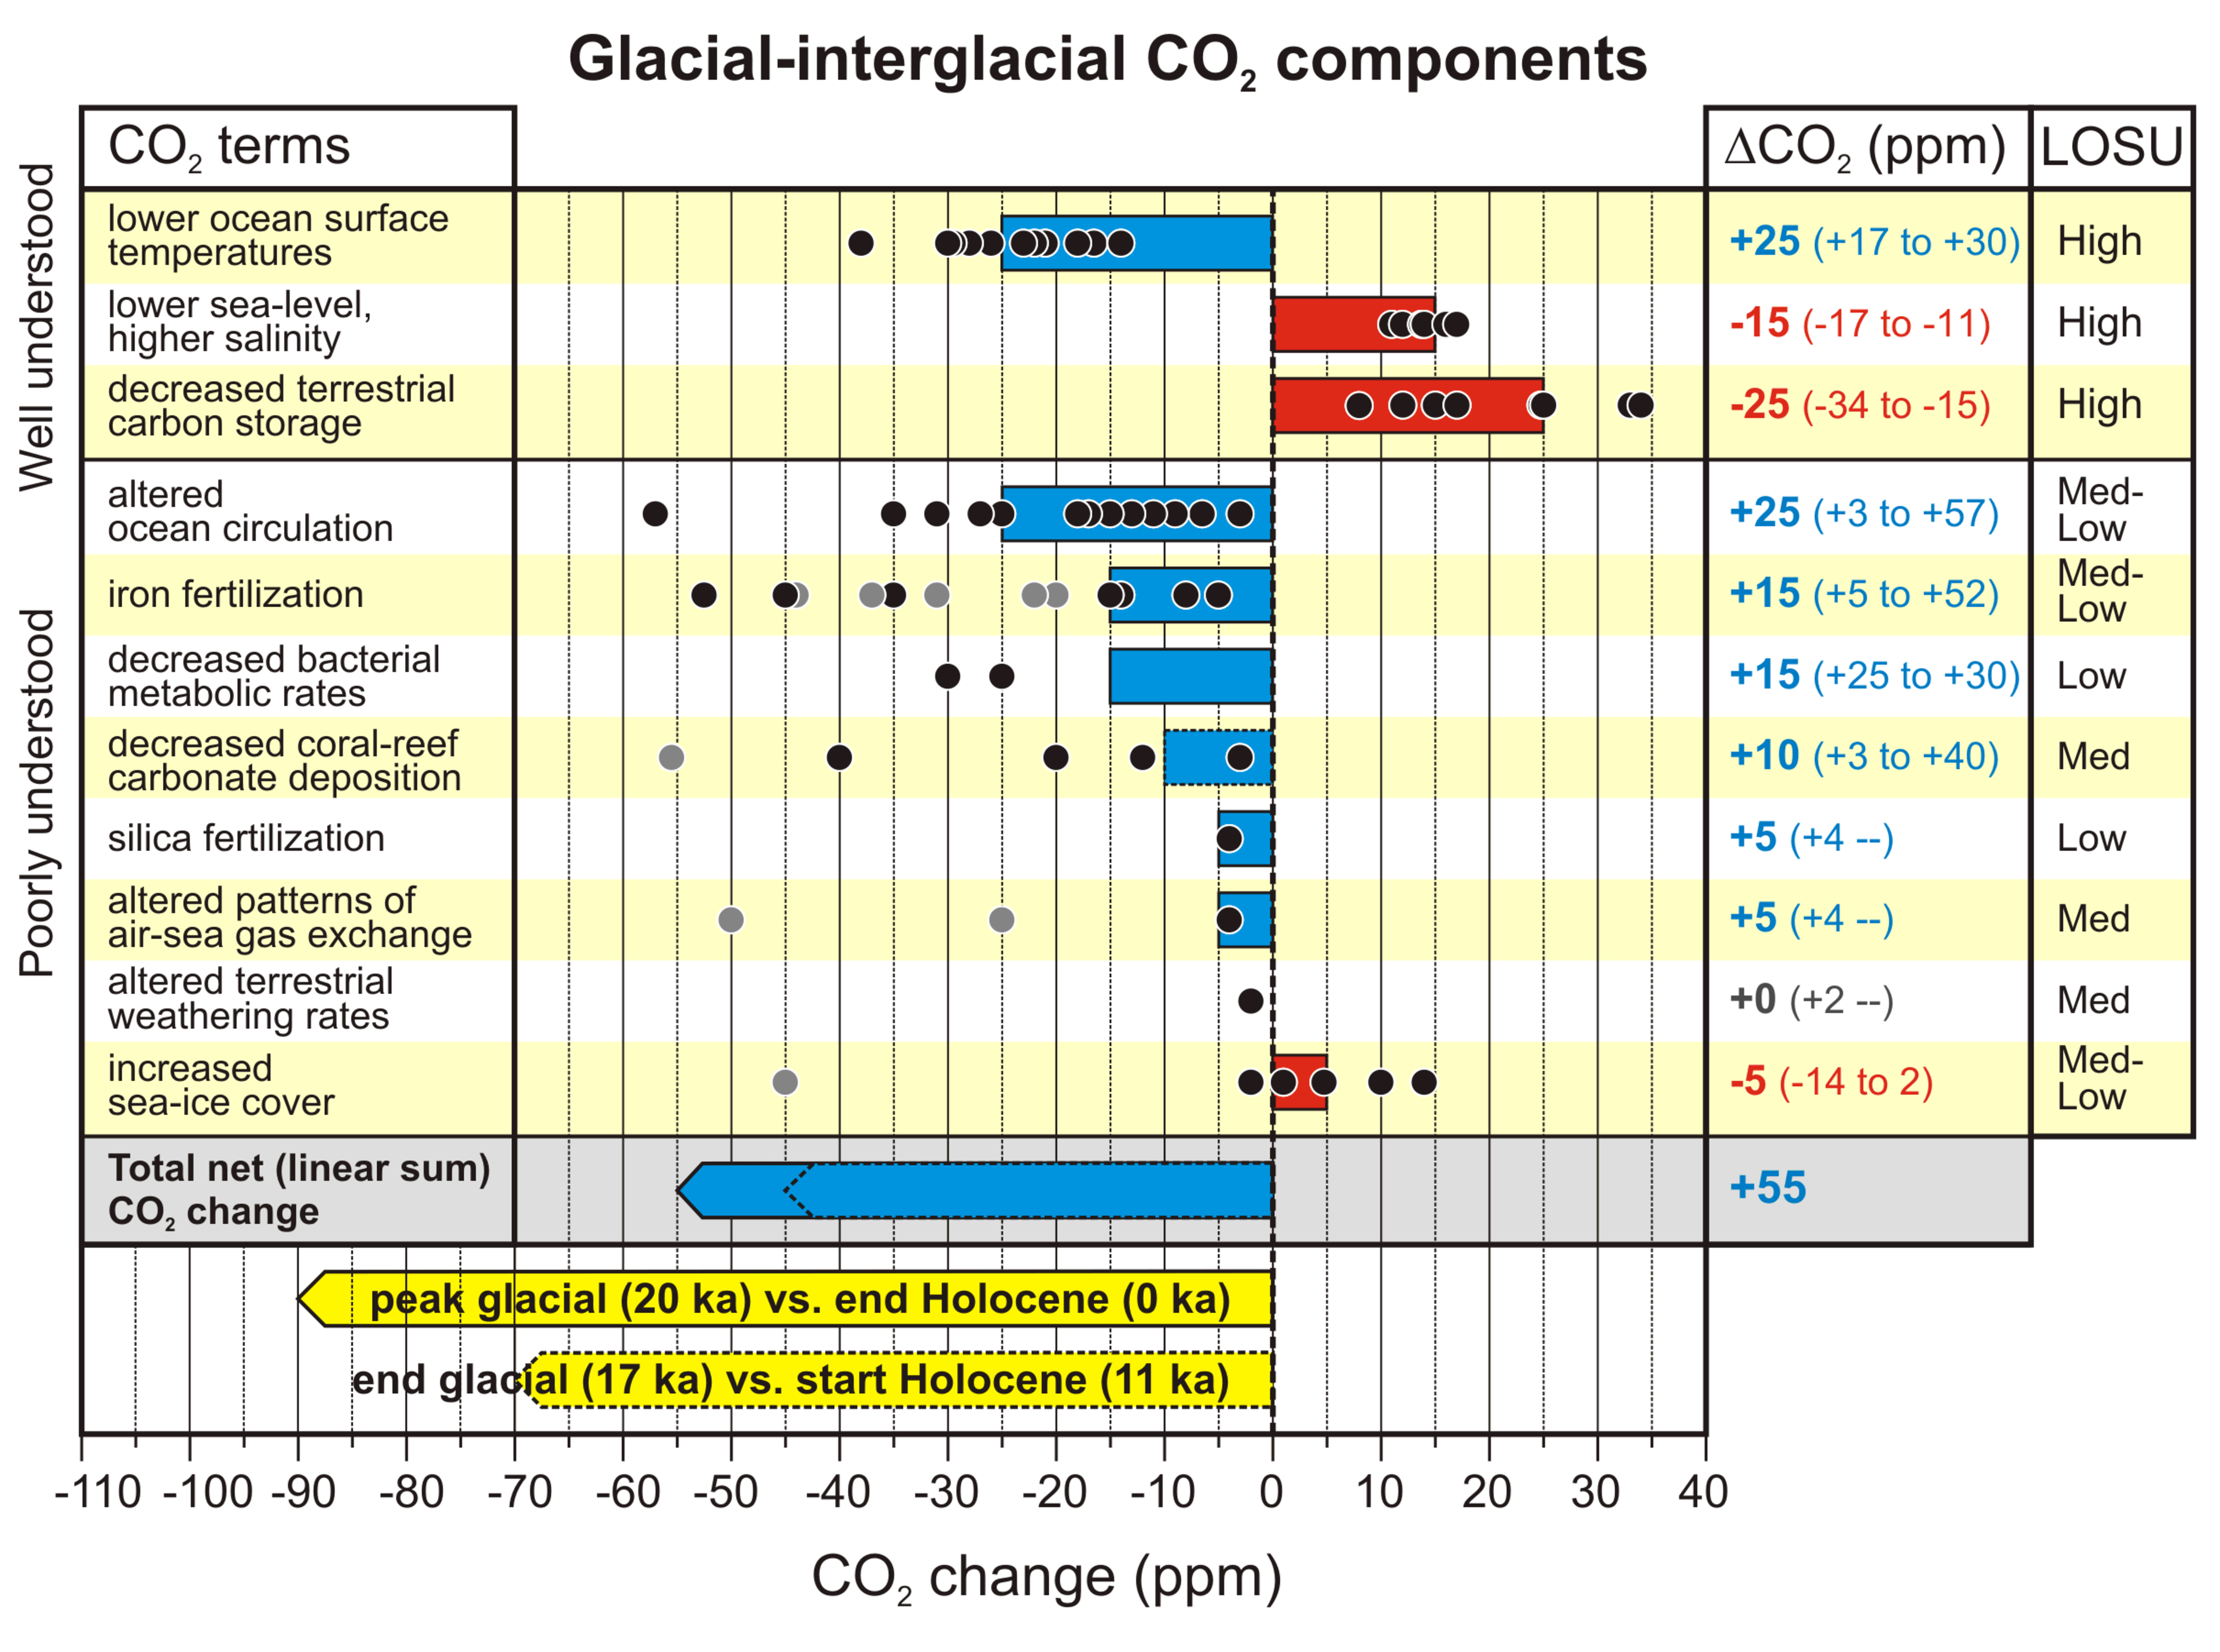
\includegraphics[width=1.00\textwidth]{CO2_components_110104.pdf}
\caption{Baaaa.}
\label{fig:CO2_components_110104}
\end{figure}

%------------------------------------------------
\newpage
%------------------------------------------------

\section{Ocean carbon geoengineering}

\noindent Another way to view and understand marine carbon and nutrient cycling and the 'biological pump' in the ocean is through the lens of geoengineering. In this Section you'll use geoengineering as an 'excuse' to perturb and elucidate the response of the global carbon cycle and climate system and hence learn something new/different about Earth system dynamics compared to e.g. its response only under standard future carbon emissions scenarios.

In the following experiments you are going to explore some of the ocean biological controls on atmospheric p\(CO_{2}\) (plus ocean acidification, and the distributions and intensities of oxygen minimum zones). Really, the ‘geoengineering’ focus is just an excuse to be looking at how the biological pump in the ocean works, how it regulates atmospheric p\(CO_{2}\), how sensitive it is to perturbation and what the consequences are of any changes in it. So if you are uncomfortable with ideas of large scale manipulating the Earth system, you might instead think about the relevance of the experiments to e.g. understanding why atmospheric p\(CO_{2}\) was low at the time of the last glacial.

The overall idea of this Chapter is to run future \(CO_{2}\) emissions scenarios and test whether ocean carbon geoengineering is an effective means for reducing future ocean acidification and marine ecological impacts (but keeping in mind that you are also exploring the basic natural operation of the system in doing so). You will require a pre-industrial \textit{spin-up} and will first need to create a new historical p\(CO_{2}\) transient experiment because you are now using a different \textit{base-config} (\texttt{cookie.CB.p\_worjh2.BASESFe}) that includes additional tracers for the marine iron cycle, i.e. you cannot simply use any of the experiments from previous labs as a \textit{re-start}. e.g. refer to Section 14.6  for a guide as to what to ‘look for’ in the model results.

%------------------------------------------------
\vspace{1mm}
\noindent\rule{4cm}{0.1mm}
\vspace{2mm}
%------------------------------------------------

\noindent To start with, go ahead and run a new historical transient experiment. A \textit{user-config} is provided for your convenience (\texttt{ch07.5.historical.EXPT}) … but maybe check the settings for e.g. start year, as well as note that there are a number of new parameters to control the iron cycle (amongst other differences) as compared to before:
\vspace{-2pt}\begin{verbatim}
$ ./runcookie.sh cookie.CB.p_worjh2.BASESFe LABS
   ch07.5.historical.EXPT 245 cookie.CB.p_worjh2.BASESFe.FeMIP.SPIN
\end{verbatim}\vspace{-2pt}
(ignore the ‘WARNING’s at the start)

%------------------------------------------------
\vspace{1mm}
\noindent\rule{4cm}{0.1mm}
\vspace{2mm}
%------------------------------------------------

\noindent The provided example \textit{user-config} -- \texttt{LAB\_4.EXAMPLE} -- includes parameter settings for controlling any one of 3 different possible ocean carbon geoengineering schemes, described below. By default, these are commented out (== ignored by the model) and only the forcing for the A2 emissions scenario (\texttt{worjh2.FeMahowald2006.FpCO2\_Fp13CO2\_A2\_02180PgC}) with no geoengineering enacted,  is enabled by default. You might regard this as a control (reference) experiment for all the with-geoengineering experiments you might run, i.e. the impacts of \(CO_{2}\) emissions in the absence of any mitigation by geoenginerring. To activate any particular geoengineering forcing: simply un-comment (delete the \# at the start of) the appropriate pair of lines (the first line being the forcing specification, and the second one the total flux forcing used in the geoengineering scheme). If you have multiple (un-commented) settings of a parameter (e.g. \texttt{bg\_par\_forcing\_name}), then the value specified in the last occurrence of the parameter, is the one that is applied. This can get confusing, so if you un-comment out one set of parameter options, comment out (add a \# to) the ones you are not using.

The geoengineering (and control) experiments need to be run starting from the end of your historical transient experiment:
\vspace{-2pt}\begin{verbatim}
$ ./runcookie.sh cgenie.eb_go_gs_ac_bg.worjh2.BASEFe LABS
   LAB_4.EXAMPLE 90 LAB_4.historical
\end{verbatim}\vspace{-2pt}
Because with a modern configuration and additional tracers in the ocean, the model is running rather slower than in some earlier exercises, you may not want to run beyond the end of the century (hence the 90 year experiment duration, starting from year 2010, as suggested above).

%------------------------------------------------
\vspace{1mm}
\noindent\rule{4cm}{0.1mm}
\vspace{2mm}
%------------------------------------------------

\noindent Each of the example geoengineering scenarios are delineated by its own specific \textit{forcing} – a set of files that live in a uniquely named sub-directory within \textsf{\footnotesize genie-forcings}. The three forcings are:

\vspace{1mm}
\begin{itemize}[noitemsep]
\item
\begin{verbatim}worjh2.FeMahowald2006.FpCO2_Fp13CO2_A2_02180PgC_FFe\end{verbatim}
\item
\begin{verbatim}worjh2.FeMahowald2006.FpCO2_Fp13CO2_A2_02180PgC_FPO4\end{verbatim}
\item
\begin{verbatim}worjh2.FeMahowald2006_FpCO2_Fp13CO2_A2_02180PgC_FALK\end{verbatim}
\end{itemize}
\vspace{1mm}

Each forcing includes the A2  SRES \(CO_{2}\) emissions scenario, with the annual emissions (\(CO_{2}\) flux) \texttt{biogem\_force\_flux\_atm\_pCO2\_sig.dat} in units of \(PgCyr^{-1}\) (== GtC yr-1), hence requiring a units conversion setting in the \textit{user-config} (\texttt{bg\_par\_atm\_force\_scale\_val\_3=8.3333e+013}) that is provided for you under the heading \texttt{\# CO2 emissions scaling}. (Ignore the carbon isotope settings.)

Each forcing also includes a prescribed dust flux to the ocean surface (the \textsf{\footnotesize FeMahowald2006} part of the directory name string). This is necessary because the model configuration you are using includes a co-limitation of biological productivity by iron (Fe) in addition to phosphate (\(PO_{4}\)). (The files associated with the dust forcing are: \textsf{\footnotesize biogem\_force\_flux\_sed\_det\_sig.dat} and \textsf{\footnotesize biogem\_force\_flux\_sed\_det\_SUR.dat} but you do not need to edit these files.) For the role of iron in controlling ocean productivity: possible starting points for background reading are: \textit{Ridgwell and Kohfeld} [2007] (PDF available form my website) or \textit{Jickells et al.} [2005] (Science).

\vspace{1mm}
The specific details of the 3 different example geoengineering scenarios are as follows:

%------------------------------------------------

\subsection{Iron fertilization}

\vspace{2mm}
\textit{Forcing}: \textsf{\footnotesize worjh2.FeMahowald2006.FpCO2\_Fp13CO2\_A2\_02180PgC\_FFe} \vspace{1mm}
\\-- a constant (with time) flux of dissolved Fe (in addition to whatever Fe dissolves into the surface ocean from the dust flux) is specified in: \texttt{biogem\_force\_flux\_ocn\_Fe\_sig.dat}. The magnitude of the applied flux is then scaled in the \textit{user-config} file by the setting:
\vspace{-1mm}
\small\begin{verbatim}
bg_par_ocn_force_scale_val_9=1.0e+09
\end{verbatim}\normalsize
\vspace{-1mm}
Note that this is simply an example total global flux. You might consider higher or lower fluxes, as well as potentially how ‘practical’ the annual production and supply of such quantities might be.

\vspace{1mm}
A spatial pattern of the flux is also defined, in the file:
\vspace{-1mm}
\small\begin{verbatim}
biogem_force_flux_ocn_Fe_SUR.dat
\end{verbatim}\normalsize
\vspace{-1mm}

An example pattern is set (see later for instructions on modifying this) with a row of grid cells  marked along the same latitude in the Southern Ocean. You do not need to retain this pattern. In choosing an alternative: think about where in the modern ocean biological productivity is thought to be at least partly limited by the availability of dissolved Fe. Remember that the model may or may not correspond with reality, i.e. it may or may not predict Fe limitation in the correct regions, which may affect your choice of location for iron fertilization.

%------------------------------------------------

\subsection{Phosphate fertilization}

\vspace{2mm}
\textit{Forcing}: \textsf{\footnotesize worjh2.FeMahowald2006.FpCO2\_Fp13CO2\_A2\_02180PgC\_FPO4} (‘macro-nutrient’ addition)
\vspace{1mm}
\\ -- a constant (with time) flux of dissolved \(PO_{4}\) is specified in: \texttt{biogem\_force\_flux\_ocn\_PO4\_sig.dat}. The magnitude of the applied flux is then scaled in the \textit{user-config} by the setting:
\vspace{-2mm}\small\begin{verbatim}
bg_par_ocn_force_scale_val_8=2.0e+12
\end{verbatim}\normalsize\vspace{-2mm}

Again, you should consider this as an example total flux. In choosing a total flux to apply, points of comparison include whatever the total weathering flux (via rivers) of phosphate to the global ocean is. Also: global phosphate (fertilizer) production, which produces an interesting potential conflict between geoengineering and food production, although there are proposals for using fertilized ocean regions for enhanced fish production.

\vspace{1mm}
A spatial pattern of the flux is also defined, in the file:
\vspace{-2mm}\small\begin{verbatim}
biogem_force_flux_ocn_PO4_SUR.dat
\end{verbatim}\normalsize\vspace{-2mm}

An example pattern has been set – here, the Equatorial Atlantic. In choosing your regions(s), think about where in the ocean (again – there may be differences between real ocean and model) productivity is currently limited by \(PO_{4}\). Also be aware of possible on-set of \(Fe\) limitation if you relieve the  \(PO_{4}\) limitation (i.e., you could potentially lose effectiveness if you supply too much  \(PO_{4}\) and instead productivity and \(CO_{2}\) draw-down is capped by a second factor). You could potentially consider  \(PO_{4}\) and \(Fe\) addition at the same time … ?

%------------------------------------------------

\subsection{Enhanced weathering}

\vspace{2mm}
\textit{Forcing}: \textsf{\footnotesize worjh2.FeMahowald2006.FpCO2\_Fp13CO2\_A2\_02180PgC\_FPO4} (alkalinity addition)
\vspace{1mm}
\\ -- a constant (with time) flux of alkalinity is specified in: \texttt{biogem\_force\_flux\_ocn\_ALK\_sig.dat}. The magnitude of the applied flux is then scaled in the \textit{user-config} by the setting:
\vspace{-2mm}\small\begin{verbatim}
bg_par_ocn_force_scale_val_12=5.0e+13
\end{verbatim}\normalsize\vspace{-2mm}

Again, another example total flux. In choosing a total flux to apply, points of comparison include whatever the total weathering flux (via rivers) of alkalinity (often described in terms of the bicarbonate ion flux) to the global ocean is. Also: global cement (lime) production. (Note that in one mole of lime: \(CaO\), you have 2 moles of alkalinity (\(Ca^{2+}\)).)

\vspace{1mm}
A spatial pattern of the flux is also defined, in the file:
\vspace{-2mm}\small\begin{verbatim}
biogem_force_flux_ocn_ALK_SUR.dat
\end{verbatim}\normalsize\vspace{-2mm}

An example pattern has been set – here, bordering the major tropical coral reefs locations in the Western Pacific. In choosing your regions(s), you might think about mitigating specific ecosystem impacts of ocean acidification, or about the feasibility of transport and proximity to abundant limestone (\(CaCO_{3}\) – the source of lime) and/or energy.

%------------------------------------------------
%------------------------------------------------

\subsection{Modifying spatial patterns}

\vspace{2mm}
The spatial patterns of an applied flux forcing to the ocean can easily be modified. The pattern is specified in a simple ASCII (plain text) file, in the file in the forcing sub-directory ending '\textsf{\footnotesize \_SUR.dat}'. The file (in this example the default Fe pattern) looks like:

\newpage

\tiny\begin{verbatim}
0.0 0.0 0.0 0.0 0.0 0.0 0.0 0.0 0.0 0.0 0.0 0.0 0.0 0.0 0.0 0.0 0.0 0.0 0.0 0.0   0   0   0   0 0.0 0.0 0.0 0.0 0.0 0.0 0.0 0.0 0.0 0.0 0.0 0.0
  0   0   0   0   0   0   0   0   0 0.0   0   0   0   0   0   0   0   0   0 0.0 0.0   0   0 0.0 0.0 0.0 0.0 0.0   0   0   0   0   0   0   0   0
  0   0   0   0   0   0 0.0 0.0 0.0 0.0 0.0 0.0   0   0   0   0   0   0   0   0 0.0 0.0 0.0 0.0 0.0 0.0   0   0   0   0   0   0   0   0   0   0
  0   0   0   0 0.0 0.0 0.0 0.0 0.0 0.0 0.0 0.0 0.0   0   0   0   0   0   0   0 0.0 0.0 0.0 0.0 0.0   0   0   0   0   0   0   0   0   0   0   0
  0   0   0   0 0.0 0.0 0.0 0.0 0.0 0.0 0.0 0.0 0.0 0.0   0   0   0   0   0   0 0.0 0.0 0.0 0.0 0.0 0.0   0   0   0   0   0   0   0   0   0   0
  0   0   0 0.0 0.0 0.0 0.0 0.0 0.0 0.0 0.0 0.0 0.0 0.0   0   0   0   0   0 0.0 0.0 0.0 0.0 0.0 0.0 0.0   0   0   0   0   0   0   0   0   0   0
  0   0   0 0.0 0.0 0.0 0.0 0.0 0.0 0.0 0.0 0.0 0.0 0.0   0   0   0   0 0.0 0.0 0.0 0.0 0.0 0.0 0.0   0 0.0 0.0   0   0   0   0   0   0   0   0
  0   0   0 0.0 0.0 0.0 0.0 0.0 0.0 0.0 0.0 0.0 0.0 0.0   0   0   0   0 0.0 0.0 0.0 0.0 0.0 0.0 0.0 0.0 0.0 0.0 0.0 0.0   0   0   0   0   0   0
  0   0 0.0 0.0 0.0 0.0 0.0 0.0 0.0 0.0 0.0 0.0 0.0 0.0 0.0   0   0   0 0.0 0.0 0.0 0.0 0.0 0.0 0.0   0   0 0.0 0.0   0   0   0   0   0   0   0
  0   0 0.0 0.0 0.0 0.0 0.0 0.0 0.0 0.0 0.0 0.0 0.0 0.0 0.0   0 0.0 0.0 0.0 0.0 0.0 0.0 0.0 0.0 0.0   0   0   0   0   0   0   0   0   0   0   0
  0   0 0.0 0.0 0.0 0.0 0.0 0.0 0.0 0.0 0.0 0.0 0.0 0.0 0.0   0 0.0 0.0 0.0 0.0 0.0 0.0 0.0 0.0 0.0   0   0   0   0   0   0 0.0 0.0   0   0   0
  0 0.0 0.0 0.0 0.0 0.0 0.0 0.0 0.0 0.0 0.0 0.0 0.0 0.0 0.0   0 0.0 0.0 0.0 0.0 0.0 0.0 0.0 0.0 0.0   0   0   0   0   0   0 0.0 0.0   0   0   0
  0 0.0 0.0 0.0 0.0 0.0 0.0 0.0 0.0 0.0 0.0 0.0 0.0 0.0 0.0 0.0   0 0.0 0.0 0.0 0.0 0.0 0.0 0.0 0.0   0   0   0   0   0   0 0.0 0.0   0 0.0 0.0
  0 0.0 0.0 0.0 0.0 0.0 0.0 0.0 0.0 0.0 0.0 0.0 0.0 0.0 0.0 0.0 0.0   0 0.0 0.0 0.0 0.0 0.0 0.0 0.0   0   0   0   0   0   0 0.0 0.0 0.0 0.0 0.0
  0 0.0 0.0 0.0 0.0 0.0 0.0 0.0 0.0 0.0 0.0 0.0 0.0 0.0 0.0 0.0 0.0 0.0   0 0.0 0.0 0.0 0.0 0.0 0.0   0   0   0   0   0   0 0.0 0.0 0.0 0.0 0.0
  0 0.0 0.0 0.0 0.0 0.0 0.0 0.0 0.0 0.0 0.0 0.0 0.0 0.0 0.0 0.0 0.0 0.0   0   0 0.0 0.0 0.0 0.0 0.0   0   0   0   0   0   0 0.0 0.0 0.0 0.0 0.0
  0 0.0 0.0 0.0 0.0 0.0 0.0 0.0 0.0 0.0 0.0 0.0 0.0 0.0 0.0 0.0 0.0 0.0   0   0 0.0 0.0 0.0 0.0 0.0 0.0 0.0   0   0   0 0.0 0.0 0.0 0.0 0.0 0.0
  0   0 0.0 0.0 0.0 0.0 0.0 0.0 0.0 0.0 0.0 0.0 0.0 0.0 0.0 0.0 0.0 0.0   0   0   0 0.0 0.0 0.0 0.0 0.0 0.0   0   0   0 0.0 0.0 0.0 0.0 0.0 0.0
  0   0 0.0 0.0 0.0 0.0 0.0 0.0 0.0 0.0 0.0 0.0 0.0 0.0 0.0 0.0 0.0 0.0   0   0   0 0.0 0.0 0.0 0.0 0.0 0.0   0   0   0 0.0 0.0 0.0 0.0 0.0 0.0
0.0   0 0.0 0.0 0.0 0.0 0.0 0.0 0.0 0.0 0.0 0.0 0.0 0.0 0.0 0.0 0.0 0.0   0   0   0   0 0.0 0.0 0.0 0.0 0.0   0   0   0 0.0 0.0 0.0 0.0 0.0 0.0
0.0   0 0.0 0.0 0.0 0.0 0.0 0.0 0.0 0.0 0.0 0.0 0.0 0.0 0.0 0.0 0.0 0.0   0   0   0   0 0.0 0.0 0.0 0.0 0.0   0   0   0 0.0 0.0 0.0 0.0 0.0 0.0
0.0 0.0   0   0 0.0 0.0 0.0 0.0 0.0 0.0 0.0 0.0 0.0 0.0 0.0 0.0 0.0 0.0   0   0   0   0 0.0 0.0 0.0 0.0 0.0   0   0   0 0.0 0.0 0.0 0.0 0.0 0.0
0.0 0.0   0   0 0.0 0.0 0.0 0.0 0.0 0.0 0.0 0.0 0.0 0.0 0.0 0.0 0.0 0.0   0   0   0   0 0.0 0.0 0.0 0.0 0.0   0   0   0 0.0 0.0 0.0 0.0 0.0 0.0
0.0 0.0   0   0 0.0 0.0 0.0 0.0 0.0 0.0 0.0 0.0 0.0 0.0 0.0 0.0 0.0 0.0 0.0   0   0   0 0.0 0.0 0.0 0.0 0.0   0   0   0 0.0 0.0 0.0 0.0 0.0 0.0
0.0 0.0   0   0   0 0.0 0.0 0.0 0.0 0.0 0.0 0.0 0.0 0.0 0.0 0.0 0.0 0.0 0.0   0   0   0 0.0 0.0 0.0 0.0 0.0   0   0 0.0 0.0 0.0 0.0 0.0 0.0 0.0
0.0 0.0   0   0   0 0.0 0.0 0.0 0.0 0.0 0.0 0.0 0.0 0.0 0.0 0.0 0.0 0.0 0.0   0   0 0.0 0.0 0.0 0.0 0.0 0.0 0.0   0 0.0 0.0 0.0 0.0 0.0 0.0 0.0
0.0 0.0   0   0   0 0.0 0.0 0.0 0.0 0.0 0.0 0.0 0.0 0.0 0.0 0.0 0.0 0.0 0.0   0   0 0.0 0.0 0.0 0.0 0.0 0.0 0.0   0 0.0 0.0 0.0 0.0 0.0 0.0 0.0
0.0 0.0 0.0   0   0 0.0 0.0 0.0 0.0 0.0 0.0 0.0 0.0 0.0 0.0 0.0 0.0 0.0 0.0   0   0 0.0 0.0 0.0 0.0 0.0 0.0 0.0   0 0.0 0.0 0.0 0.0 0.0 0.0 0.0
0.0 0.0 0.0 0.0   0 0.0 0.0 0.0 0.0 0.0 0.0 0.0 0.0 0.0 0.0 0.0 0.0 0.0 0.0   0 0.0 0.0 0.0 0.0 0.0 0.0 0.0 0.0 0.0 0.0 0.0 0.0 0.0 0.0 0.0 0.0
0.0 0.0 0.0 0.0 0.0 0.0 0.0 0.0 0.0 0.0 0.0 0.0 0.0 0.0 0.0 0.0 0.0 0.0 0.0   0 0.0 0.0 0.0 0.0 0.0 0.0 0.0 0.0 0.0 0.0 0.0 0.0 0.0 0.0 0.0 0.0
0.0 0.0 0.0 0.0 0.0 0.0 0.0 0.0 0.0 0.0 0.0 0.0 0.0 0.0 0.0 0.0 0.0 0.0 0.0   0 0.0 0.0 0.0 0.0 0.0 0.0 0.0 0.0 0.0 0.0 0.0 0.0 0.0 0.0 0.0 0.0
0.0 0.0 0.0 0.0 0.0 0.0 0.0 0.0 0.0 0.0 0.0 0.0 0.0 0.0 0.0 0.0 0.0 0.0 0.0   0 0.0 0.0 0.0 0.0 0.0 0.0 0.0 0.0 0.0 0.0 0.0 0.0 0.0 0.0 0.0 0.0
0.0 0.0 0.0 0.0 0.0 0.0 0.0 0.0 0.0 0.0 0.0 0.0 0.0 0.0 0.0 0.0 0.0 0.0 0.0 0.0 0.0 0.0 0.0 0.0 0.0 0.0 0.0 0.0 0.0 0.0 0.0 0.0 0.0 0.0 0.0 0.0
1.0 1.0 1.0 1.0 1.0 1.0 1.0 1.0 1.0 1.0 1.0 1.0 1.0 1.0 1.0 1.0 1.0 1.0 1.0 1.0 1.0 1.0 1.0 1.0 1.0 1.0 1.0 1.0 1.0 1.0 1.0 1.0 1.0 1.0 1.0 1.0
  0 0.0 0.0 0.0 0.0 0.0 0.0 0.0 0.0 0.0 0.0 0.0 0.0 0.0 0.0 0.0 0.0 0.0 0.0 0.0 0.0 0.0 0.0 0.0 0.0 0.0 0.0 0.0 0.0 0.0 0.0 0.0 0.0 0.0 0.0   0
  0   0   0   0   0   0   0   0   0   0   0   0   0   0   0   0   0   0   0   0   0   0   0   0   0   0   0   0   0   0   0   0   0   0   0   0
\end{verbatim}\normalsize

Here: ‘\texttt{0}’s represent land and cannot have a forcing associated with them. ‘\texttt{0.0}’s represent a zero flux to the ocean, and ‘\texttt{1.0}’s the default Southern Ocean forcing pattern. Note that a distinction is made between a ‘\texttt{0}’ and a ‘\texttt{0.0}’ so that you can make out where the continents are and do not necessarily have to count in the \textit{i} and \textit{j} grid directions to find a specific location. The grid is the same as you saw previously in tracing ocean circulation, and which numbered the \textit{i} and \textit{j} axes if that helps. For the ALK forcing, ‘\texttt{1.0}’s are set off of the coast of Australia and SE Asia and in the \(PO_{4}\) forcing, in the Atlantic.

There is no more to changing the pattern of the flux forcing than simply marking with a ‘\texttt{1.0}’ where you would like the forcing applied, and a ‘\texttt{0.0}’ where it should not be. Note that there should be a single blank line at the bottom of the file. (If you have problems applying a modified spatial pattern – check that this is present.) Copy the entire \textit{forcings} directory and rename each time to create a new pattern, remembering to change the name of the \textit{forcing} in the \texttt{bg\_par\_forcing\_name} parameter. ( is best to keep a copy of the original forcing in case you make a mess of the spatial pattern file, but the original can also be recovered from the code server.)

%------------------------------------------------
%------------------------------------------------

\subsection{Impacts to look out for}

\begin{itemize}

\vspace{1mm}
\item Impacts and ecosystems of interest could potentially be ones residing on the ocean floor, such as cold-water (deep water) corals, and are not necessarily planktic (/surface) only.

\vspace{1mm}
\item Don’t forget that different calcifying organisms employ different mineralogies (calcite vs. aragonite), with different saturation states and hence potentially susceptibility to ocean acidification. Hence thresholds of both aragonite and calcite saturation will be relevant, depending on the organism. Depending on the organism, saturation changes occurring in specific regions may much more relevant than a global mean change. Also, it might be the seasonal minimum value reached, rather than annual averaged minimum, that is critical.

\vspace{1mm}
\item Some of the arguments against some forms of ocean carbon geoengineering concern the potential for adverse impacts on marine organisms (and positive climate feedbacks) induced by decreases in the degree of oxygenation in the ocean, such as expanding and/or intensifying oxygen minimum zones. \textbf{cookie} saves 3D fields of \(O_{2}\) concentrations that can be plotted in slices through the ocean of various orientations.

\end{itemize}





\begin{figure}[ht]
\begin{center}
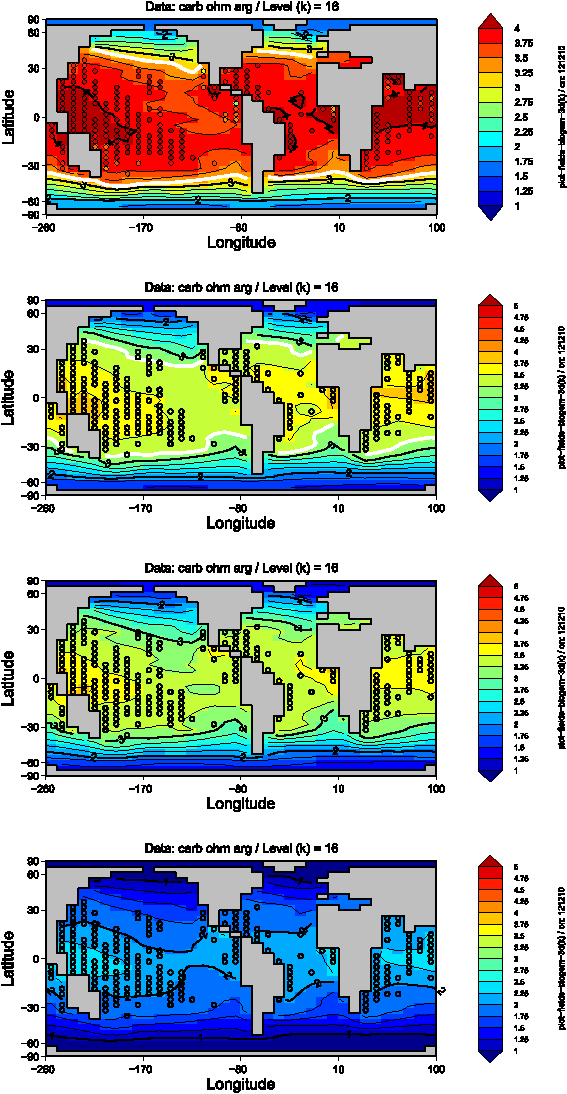
\includegraphics[scale=0.875]{chx-oaimpacts.pdf}
\end{center}
\caption{
\textbf{Mean annual ocean surface saturation (aragonite) changes.}
Top: pre-industrial model ocean surface saturation (aragonite) with ReefBase tropical coral reef locations re-gridded to the \textbf{cookie} grid and color-coded with modern observationally-based saturation values.
2nd and 3rd down: Year 1994 and 2010 ocean surface saturation (aragonite) with ReefBase reef locations.
Bottom: Year 2010 ocean surface saturation (aragonite) under the A2 \(CO_{2}\) emissions scenario.
The thick white line delineates the 3.25 saturation contour (inferred to reflect a limitation on corals).
\textit{Examples here produced using \textbf{cookieplot} but equally do-able in \textbf{Panoply} with the exception of achieving a data overlay. These are provided simply to illustrate some of the impacts you might consider and possible ways of visualizing them.}
}
\label{fig:chx-oaimpacts}
\end{figure}

\begin{figure}[ht]
\begin{center}
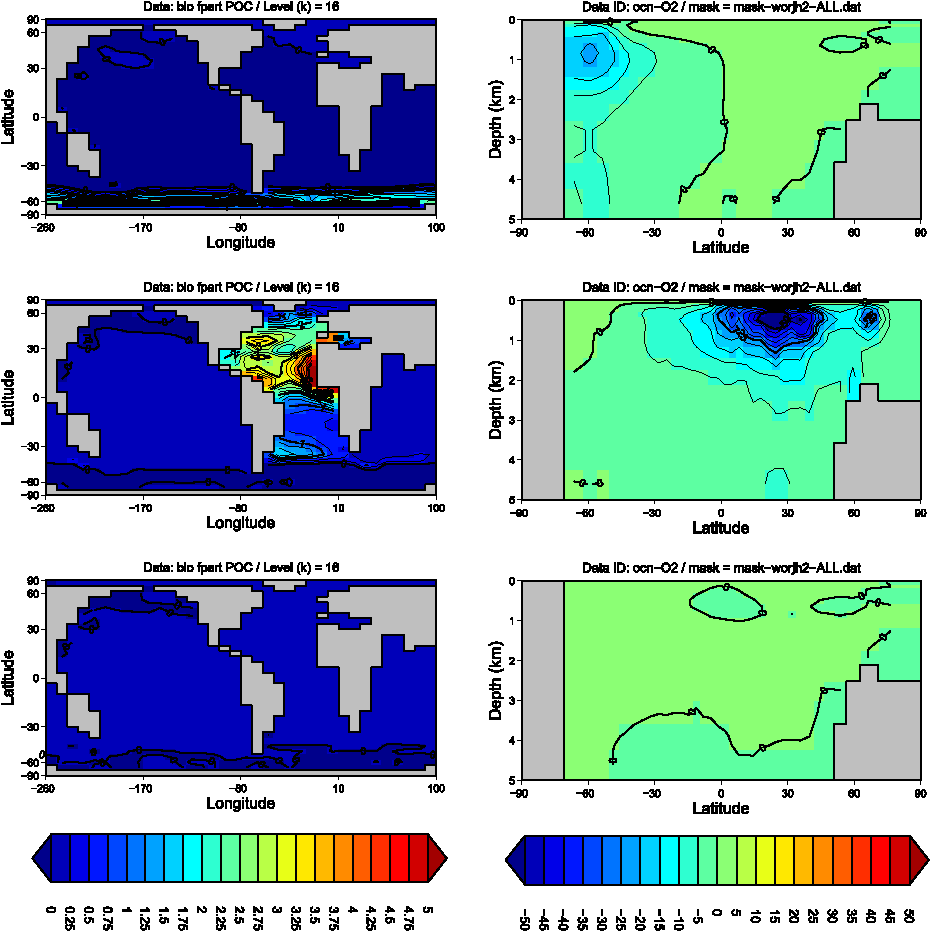
\includegraphics[scale=0.875]{chx-geoengimpacts.pdf}
\end{center}
\caption{
\textbf{Ocean surface export (particulate organic carbon) and zonal \([O_{2}]\) anomalies.}
Left: anomalies of global mean annual export production, for \(Fe\) fertilization (top), \(PO_{4}\) addition (middle), and ocean liming (bottom).
Right: Zonal mean anomalies of dissolved \(O_{2}\) concentrations.
\textit{Examples here produced using \textbf{cookieplot} but equally do-able in \textbf{Panoply} with the exception of achieving a data overlay. These are provided simply to illustrate some of the impacts you might consider and possible ways of visualizing them.}
}
\label{fig:chx-geoengimpacts}
\end{figure}





%----------------------------------------------------------------------------------------
%----------------------------------------------------------------------------------------